\subsection*{2.b.1 Calcolare la "resistenza di irraggiamento" di un circuito elettrico quadrato di lato L, piccolo rispetto alla lunghezza d'onda $\lambda$ della radiazione monocromatica incidente, se il circuito è puramente resistivo con resistenza R.\\
Calcolare anche la sezione d'urto di assorbimento e la sezione d'urto elastica se l'onda incidente ha campo magnetico perpendicolare al piano del circuito e di modulo massimo $B_0$. }
Nomi a parte il problema è schematizzato in Figura:
\begin{figure}[H]
	\centering
	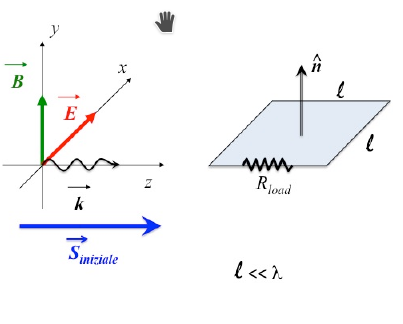
\includegraphics[width=0.5\textwidth]{immagini/spira_onda.png}
	\caption{Spira immersa nel campo di onda e.m.}
	\label{fig:spira1}
\end{figure}
\paragraph{Calcolo della resistenza di irraggiamento.}
I campi ed il vettore di Poynting dell'onda sono:
\[
	\boldsymbol{E} = E_x \hat{i} = E_0 \cos\left( \omega t - kz \right) \hat{i} 
.\] 
\[
	\boldsymbol{B} = B_y \hat{j} = B_0 \cos\left( \omega t - kz \right) \hat{j} 
.\] 
\[
	\boldsymbol{S}_{in} = \frac{E_0^2}{Z_0}\cos\left( \omega t - kz \right) \hat{k} 
.\] 
Sia $I\left( t \right) $ la corrente che scorre nel circuito; possiamo sfruttare le ipotesi di dimensioni piccole (rispetto a $\lambda$) per dire che tale corrente è uniforme in tutta la spira. Trascurando anche autoinduttanza e capacità parassite possiamo affermare che il circuito ha momento di dipolo nullo.\\
Non vale lo stesso per il momento di dipolo magnetico:
\[
	\boldsymbol{p}_m = I\left( t \right) l^2 \hat{j}
.\] 
Adesso aggiungendo le ipotesi di perfetta monocromaticita dell'onda incidente e di nessuna perdita di energia per irraggiamento del circuito si calcola la corrente $I\left( t \right)$ applicando Faraday:   
\[
	\varepsilon\left( t \right) = - \frac{\mbox{d} \Phi\left( \boldsymbol{B} \right) }{\mbox{d} t} = R_{load} I\left( t \right) 
.\]
Mettiamo quindi in mezzo la geometria del circuito:
\[
	I\left( t \right) = \frac{\varepsilon\left( t \right)}{R_{load}} = 
	- \frac{1}{R_{load}} \frac{\mbox{d} \Phi\left( \boldsymbol{B} \right) }{\mbox{d} t} 
	= - \frac{1}{R_{load}} \frac{\mbox{d}}{\mbox{d}t} \left[ \int_{-l/2}^{l/2} B_0 \cos\left( \omega t - kz \right) l dz \right] 
	= \frac{\omega l^2B_0\sin\left( \omega t\right)}{R_{load}} \frac{\sin\left( kl/2 \right)}{kl/2}      
.\] 
Agginungendo l'approssimazione:
\[
	\frac{kl}{2} = \frac{\pi l}{\lambda} \ll 1 \implies I\left( t \right) = \frac{\omega l^2 B_0 \sin\left( \omega t \right) }{R_{load}}  
.\] 
Possiamo allora calcolare la potenza irraggiata:
\[
	P_{el} = \frac{\left| \ddot{\boldsymbol{p_m}} \right| ^2}{6\pi \epsilon_0 c^{5}} = \frac{\ddot{I}^2\left( t \right) l^4}{6\pi \epsilon_0 c^5}
.\] 
Se si effettua un bilancio energetico del circuito:
\[
	\varepsilon I = R_{load}I^2 + P_{el} = R_{load} I^2 + \frac{l^4}{6\pi \epsilon_0 c^5}\ddot{I}^2
.\] 
Nel caso in analisi la f.e.m. è armonica 
\[
	\varepsilon = \varepsilon_0 \sin\left( \omega t \right) \quad 
	\text{ con } \quad  
	\varepsilon_0 = \omega l^2 B_0
\]
Quindi la soluzione stazionaria per la corrente sarà anch'essa armonica: $I = I_0 \sin\left( \omega t \right) $, in conclusione:
\[
	\varepsilon I = R_{load}I^2 + \frac{\omega ^{4}l^{4}}{6\pi \epsilon_0 c^{5}} \implies \varepsilon = \left( R_{load} + R_{irr} \right) I
.\] 
Dove è stata definita la resistenza di irraggiamento (dipendente dalla frequenza):
\[
	R_{irr} = \frac{\omega^4l^4}{6\pi \epsilon_0 c^5}
.\]
Espressa in funzione della lunghezza d'onda:
\[
	R_{irr} = \omega^4 \frac{l^4}{6\pi \epsilon c^5} = \left( \frac{2\pi c}{\lambda} \right) ^4 \frac{l^4\sqrt{\mu_0 \epsilon_0} }{6 \pi \epsilon_0 c^4} = \frac{8}{3}\pi^3 Z_0\left( \frac{l}{\lambda} \right)^4 = 31.1 \text{ k}\Omega \left( \frac{l}{\lambda} \right)^4  
.\] 
\paragraph{Calcolo delle sezioni d'urto.}
Notando che 
\[
	I\left( t \right) = \frac{\varepsilon\left( t \right) }{\left( R_{load} + R_{irr} \right) }
.\] 
Possiamo ottenere la potenza assorbita e la potenza "elastica":
\[
	P_{abs} = R_{load} I^2 = \frac{R_{load}}{\left( R_{load} + R_{irr} \right) ^2}\varepsilon^2
.\] 
\[
P_{el} = R_{irr} I^2 =  \frac{R_{load}}{\left( R_{load} + R_{irr} \right) ^2}\varepsilon^2
.\] 
Quindi la potenza trasferita al carico è massima per $R_{load} = R_{irr}$.\\
Adesso basta mediare il vettore di Poynting per concludere:
\[
\left< \left| \boldsymbol{S}_{in} \right| \right> = \frac{\boldsymbol{E}_0^2}{2Z_0}
.\] 
llora le sezioni d'urto sono:
\[
	\sigma_{abs} = \frac{4\pi^2}{\lambda^2}l^4Z_0 \frac{R_{load}}{\left(R_{load} + R_{irr}\right)^2}
.\] 
\[
	\sigma_{irr} = \frac{4\pi^2}{\lambda^2}l^4Z_0 \frac{R_{irr}}{\left(R_{load} + R_{irr}\right)^2}
.\]
\[
	\sigma_{tot} = \sigma_{irr} + \sigma_{load} = \frac{4\pi^2}{\lambda^2}l^4Z_0 \frac{Z_0}{\left(R_{load} + R_{irr}\right)^2}
.\] 

\subsection*{2.b.2 Utilizzando le apposite tabelle che forniscono le masse dei nuclei, determinare il Q-valore o l'energia di soglia dei seguenti processi, valutando l'eventuale ruolo della interazione coulombiana nello stato iniziale:
\begin{enumerate}	
	\item	p + 40Ar $\implies$ p + 39Ar + n 
	\item	p + 14N $\implies$ X + n
	\item	p + 16O $\implies$ X + n
	\item	n + 14N $\implies$ 14C + p
	\item	4He + 14N $\implies$ 17O + p
	\item	2H + 3H $\implies$ 4He + n
	\item	2H + 2H $\implies$ 4He + $\gamma$
	\item	p + 198Hg $\implies$ 197Au + p + p
\end{enumerate}
}
Partiamo con un pò di teoria:
\[
	Q = \sum M_{in} - \sum M_{fin} 
.\] 
Se il Q-valore è positivo allora la reazione avviene in modo spontaneo: l'energia di soglia è nulla.\\
Se il Q-valore è negativo allora l'energia di soglia è maggiore di zero e dipende dalla carica del proiettile.
Se la particella proiettile è neutra allora l'energia di soglia è il modulo del Q-valore, altrimenti è necessario calcolare l'energia necessaria a vincere l'interazione columbiana per arrivare al nucleo (essendo le interazioni sopra scritte tutte forti) nel sistema del laboratorio.\\
Per effettuare il calcolo sfruttiamo la conservazione dell'energia e della quantità di moto non relativistiche in una dimensione, chiariamo la notazione:
\begin{itemize}
	\item $R$: raggio del nucleo colpito 
	\item $m_{prt}$: massa del proiettile.
	\item v$_0$: velocità iniziale del proiettile.
	\item $T$: energia cinetica iniziale del proiettile.
	\item $Z$: protoni del nucleo colpito.
	\item  $M$: massa del nucleo colpito.
	\item $d$: distanza in cui i nuclei si urtano definita dalla somma dei raggi delle due particelle coinvolte:
		 \[
			 d = R + r_{prt} \approx \left( 1.25 A^{1/3} + r_{\text{skin}} + r_{prt} \right) \text{ fm} = \left( 1.25 A^{1/3} + 2 + r_{prt} \right) \text{ fm}  
		.\] 
\end{itemize}
Facendo il conto:
 \[
\begin{cases}
	m_{prt}\text{v}_0 = \left( m_p + M \right)V_{cm}\\
	T \ge \frac{1}{2}\left( m_{prt} + M \right)V_{cm} + \frac{Ze^2}{4\pi \epsilon_0 d} \\
	T = \frac{1}{2}m_{\text{prt}}\text{v}_0^2
\end{cases}
\]
Quindi sviluppando per $T$ si ottinene l'energia cinetica necessaria per la reazione:
\[
	T \ge \left( 1 + \frac{m_{prt}}{M} \right) \frac{Ze^2}{4\pi \epsilon_0 d} = T_{\text{min}} 
.\] 
e per l'energia di soglia dobbiamo soltanto sommare il modulo del Q-valore:
\[
	E_{\text{soglia}} = T_{\text{min}} + \left| Q \right| 
.\] 
In questo modo possiamo risolvere tutte le interazioni elencate.

\subsection*{2.b.3  Dimostrare la relazione fra la definizione della sezione d’urto elastica nel caso di fotoni incidenti su un unico bersaglio e la definizione di sezione d'urto elastica per un’onda e.m. monocromatica su un unico bersaglio.}

\subsection*{2.b.4  Quale calcolo si deve effettuare per determinare il numero di eventi per unità di tempo e di volume che si producono negli urti fra particelle di due specie diverse e differenti concentrazioni le cui velocità relative sono distribuite con un funzione $f(V_{rel})$, normalizzata all'unità, e la cui sezione d'urto è $\sigma(V_{rel})$?}

\subsection*{2.b.5 Calcolare l'attenuazione di un fascio di particelle incidenti su un materiale omogeneo e composto da atomi di una sola specie in funzione della profondità [dati: sezione d'urto del processo su ogni atomo del bersaglio, densità di massa del mezzo, numero atomico del mezzo].}

\subsection*{2.b.6  Calcolare l'attenuazione di un fascio di particelle incidenti su un materiale omogeneo e composto da atomi di diverse specie in funzione della profondità [dati: sezione d'urto del processo su ogni atomo del bersaglio, densità di massa del mezzo, numeri atomici, composizione chimica del mezzo]}

\subsection*{2.b.7  Effettuare una stima numerica della sezione d'urto totale forte per i seguenti urti: 
\begin{enumerate}
	\item	p + 40Ar
	\item	n + 14N
	\item	4He + 14N
	\item	2H + 3H
\end{enumerate}
}

\subsection*{2.b.8  Calcolare l’energia che dovrebbe avere un protone che incide su un protone fermo per ottenere una energia nel centro di massa pari a quella di LHC (14TeV) Calcolare l’energia degli elettroni/positroni per innescare la reazione $reazione!$ in cui i due leptoni collidono con 3-impulsi opposti, ma di modulo diverso.}

\subsection*{2.b.9 Calcolare l'energia di degli elettroni/positroni per innescare la reazione:
\[
	e^{+} \ + \ e^{-} \implies p \ + \ \overline{p}
\] 
in cui i due leptoni collidono con 3-impulsi opposti e di modulo diverso.}

\subsection*{2.b.10 Calcolare l’energia di soglia nel laboratorio per le seguenti reazioni (la seconda particella è inizialmente ferma):
\begin{enumerate}
	\item	$\gamma \ + \ {}^{16} O \implies e^{+} \ + \ e^{-} \ + \ {}^{16}O $
	\item	$\gamma \ + \ e^{-} \implies e^{-} \ + \ e^{+} \ + \ e^{-}$
	\item	$p \ + \ p \implies p \ + \ p \ + \ p \ + \ \overline{p}$
	\item	$p \ + \ {}^{16}O \implies p \ + \ p \ + \ \overline{p} \ + \ {}^{16}O$
	\item	$e^{+} \ + \ e^{-} \implies p \ + \ \overline{p}$
	\item	$e^{-} \ + \ p \implies n \ + \ \nu_e$
	\item	$\overline{\nu_e} \ + \ p  \implies n \ + \ e^{+}$
\end{enumerate}
}

\subsection*{2.b.11 Calcolare la probabilità che un neutrino interagisca nell’attraversare la Terra lungo un diametro.\\
Nota: sia assuma che l’energia del neutrino sia tale che la sezione d’urto totale su un singolo nucleone sia 1 fb. } 

\subsection*{2.b.12 Dimostrare che un elettrone (non relativistico) soggetto ad una forza elastica di richiamo, ad una forza di attrito viscoso ed alla forza di reazione radiativa, nel campo di un’onda e.m. piana polarizzata linearmente oscilla con la legge:
\[
	\boldsymbol{x} = \frac{e \boldsymbol{E_0}}{m_{e}} \frac{1}{\omega_0^2-\omega^2-i\omega\Gamma_{tot}} e^{-i \omega t} \quad \quad 
	\text{ con }  \quad \quad
	\Gamma_{tot} = \Gamma' + \Gamma \frac{\omega^2}{\omega_{0}^2}
\] 
}

\subsection*{2.b.13 Dimostrare che la sezione d’urto differenziale elastica per un’onda e.m. piana e monocromatica su un elettrone legato elasticamente vale 
\[
	\frac{\mbox{d} \sigma_{el}}{\mbox{d} \Omega} = r_e^2 L\left( \omega \right) \sin^2\left( \alpha  \right)    
\]
con $\alpha$ angolo fra la direzione di osservazione e direzione di polarizzazione (lineare) dell'onda.}

\subsection*{2.b.14 Dimostrare che la sezione d’urto Thomson vale $\sigma_{Th} = \frac{8}{3}\pi r_{e}^2  = 0.66 \text{ barn}$.}

\subsection*{2.b.15 Dimostrare che la sezione d’urto elastica per un’onda e.m. piana e monocromatica su un elettrone legato elasticamente vale:
\[
	\sigma_{el} = \sigma_{Th} L\left( \omega \right) 
\] 
}

\subsection*{2.b.16. Dimostrare che la sezione d’urto totale per un’onda e.m. piana e monocromatica su un elettrone legato elasticamente vale:
\[
		\sigma_{el} = 4 \pi r_{e} c L\left( \omega \right)
\] 
}
\subsection*{2.b.17. Dimostrare che la sezione d’urto elastica per un’onda e.m. piana e monocromatica su un elettrone legato elasticamente in prossimità di una risonanza stretta (specificare il criterio) si può approssimare con una curva lorentziana
\[
	\sigma_{el} = \sigma_{Th} \frac{\omega_{0}^2 / 4}{ \left( \omega_0 - \omega \right)^2 + \frac{ \left( \Gamma' + \Gamma  \right)^2 }{4} }
\] 
}

\subsection*{2.b.18. Dimostrare che per un’onda e.m. piana e monocromatica su un elettrone legato elasticamente le sezioni d'urto al picco valgono:
\[
	\sigma_{el} = \frac{3 \lambda_{0}^2}{2 \pi} \left( \frac{\Gamma}{\Gamma + \Gamma'} \right)^2 
\]
\[
	\sigma_{TOT} = \frac{3 \lambda_{0}^2}{2 \pi} \frac{\Gamma}{\Gamma + \Gamma'}
\]
\[
	\sigma_{inel} = \frac{3 \lambda_{0}^2}{2 \pi} \frac{\Gamma \Gamma'}{\left( \Gamma + \Gamma' \right)^2 } 
\]
Con $\lambda_{0} = \frac{2 \pi c}{\omega_{0}}$
}

Perché non sale?
\subsection*{2.b.19 Dimostrare che un elettrone (moto non relativistico) soggetto ad una forza elastica di richiamo, ad una forza di attrito viscoso ed alla forza di reazione radiativa, se viene lasciato libero di oscillare da una posizione iniziale perde energia con una 1 legge esponenziale in cui la costante tempo vale $\frac{1}{\Gamma' + \Gamma}$. Come si chiama questa costante tempo? Quale sarebbe la costante tempo con cui, invece, si smorza l'ampiezza delle oscillazioni?}

\subsection*{2.b.20 Calcolare la relazione tra parametro d'impatto (b) e angolo di scattering ($\theta$) nel caso di scattering di Rutherford (Coulombiano) e di scattering su sfera rigida.} 

\subsection*{2.b.21 Calcolare la minima distanza fra le due particelle in uno scattering Rutherford.}

\subsection*{2.b.22 Calcolare l'energia minima affinché un protone possa avere una interazione forte "toccando" un nucleo di ${}^{12}C$ o di ${}^{28} Si$.}

\subsection*{2.b.23 Discutere le differenze tra lo scattering di Rutherford (particelle $\alpha$ su nuclei) e lo scattering di elettroni su bersaglio puntiforme.}

\subsection*{2.b.24 Cercando i dati nelle apposite tabelle (reperibili sul web ) si indichino gli stati finali e si calcoli il Q-valore per i decadimenti delle seguenti specie instabili: ${}^8B, {}^{39}Ar, {}^{7}Be, {}^{64}Cu, {}^{76}Ge$. }

\subsection*{2.b.25 Cercando i dati nelle apposite tabelle (reperibili sul web) si trovino i Q-valori per le reazioni 
\begin{enumerate}
	\item $n + {}^{154}Gd \implies \gamma + {}^{155}Gd$ 
	\item $n + {}^{155}Gd \implies \gamma + {}^{156}Gd$
\end{enumerate}
}

\subsection*{2.b.26 Dimostrare che $\frac{d^3 p  }{2E}$ è un invariante relativistico effettuando esplicitamente la 2Etrasformazione di Lorentz (si consideri il boost lungo un asse, p. es. l'asse x)}

\subsection*{2.b.27 Dimostrare che $d^{4}p \delta\left( p^2-m^2 \right) \theta\left( p_0 \right) = \frac{d^3 p }{2E}$  e sfruttare questo risultato per semplificare la scrittura dell’elemento infinitesimo dello spazio dei 4-impulsi di N particelle emergenti dopo la collisione di due particelle (oppure dopo il decadimento di una particella).}

\subsection*{2.b.28 Dimostrare che nel centro di massa l’elemento infinitesimo dello spazio dei 4-impulsi, nel caso di 2 sole particelle nello stato finale, si scrive come $\frac{|\boldsymbol{p_{cm}}}{4\sqrt{s}} d\Omega_{cm}.$}

\subsection*{2.b.29 Nel caso di 3 particelle nello stato finale di una reazione, dimostrare che fra il quadrato della massa invariante di due di esse e l'energia della terza (nel centro di massa) sussite una relazione lineare.}

\subsection*{2.b.30 Come si trasforma una funzione di distribuzione del 3-impulso $f\left( \boldsymbol{p} \right)d^3 \boldsymbol{p}$ di una
particella per una trasformazione di Lorentz?}

\subsection*{2.b.31 Come si trasforma una funzione di distribuzione nello spazio delle fasi 
\[
	f\left(\boldsymbol{p},\boldsymbol{r}\right)d^3 \boldsymbol{p} \ d^3 \boldsymbol{r} 
\]
di una particella per una trasformazione di Lorentz?}

\subsection*{2.b.32 Dimostrare che se la probabilità di decadimento di una particella per unità di tempo non dipende dal tempo, la probabilità di trovare la particella non decaduta al tempo t segue una legge esponenziale.}

\subsection*{2.b.33 Dire quali fra le seguenti particelle sono soggette ad interazioni forti: $ p, \overline{p} $, $\pi^{+}, \pi^{-}, \mu^{+}, \mu^{-}, e^{+}$, $e^{-}$, $\alpha,$ Nucleo di Azoto, $\nu, \overline{\nu}$ }

\subsection*{2.b.34 Pioni neutri, di energia E nel sistema del laboratorio, decadono in due fotoni. La distribuzione è isotropa ne centro di massa. Si calcoli la distribuzione dell’energia di uno dei due fotoni nel laboratorio e gli angoli, rispetto alla direzione di volo del pione, dei due fotoni nel sistema del laboratorio in funzione dell’angolo nel sistema del centro di massa.}

\subsection*{2.b.35 Calcolare la funzione di distribuzione in energia ed in angolo nel sistema del laboratorio di un fascio di neutrini o di muoni prodotto nel decadimento di pioni carichi di energia 14 GeV.}

\subsection*{2.b.36 Qual e' l'andamento delle masse nucleari a parità di A in funzione di Z?}

\subsection*{2.b.37 Dimostrare che in un tipico decadimento $\alpha$, la particella $\alpha$ emerge con circa il 98\% dell'energia disponibile.}

\subsection*{2.b.38 Dimostrare che in un decadimento $\beta$ la somma delle energie dell'elettrone e dell'antineutrino emessi é praticamente uguale al Q-valore della reazione.}
